%%% Template originaly created by Karol Kozioł (mail@karol-koziol.net) and modified for ShareLaTeX use

% \documentclass[a4paper,11pt]{article}
\documentclass[a4paper,11pt]{article}

\usepackage[english]{babel}
\usepackage{hyperref}
\usepackage[T1]{fontenc}
\usepackage[utf8]{inputenc}
\usepackage{graphicx}
\usepackage{xcolor}
\usepackage{xcolor}
\usepackage[linesnumbered, boxed,ruled,vlined]{algorithm2e}
\usepackage{algpseudocode}

\renewcommand\familydefault{\sfdefault}
\usepackage{tgheros}
% \usepackage[defaultmono]{droidmono}

\usepackage{amsmath,amssymb,amsthm,textcomp}
\usepackage{enumerate}
\usepackage{multicol}
\usepackage{tikz}

\usepackage{geometry}
\geometry{left=10mm,right=15mm,%
bindingoffset=5mm, top=15mm, bottom=20mm}


\linespread{1.3}

\newcommand{\linia}{\rule{\linewidth}{0.5pt}}

% custom theorems if needed
\newtheoremstyle{mytheor}
{1ex}{1ex}{\normalfont}{0pt}{\scshape}{.}{1ex}
{{\thmname{#1 }}{\thmnumber{#2}}{\thmnote{ (#3)}}}

\theoremstyle{mytheor}
\newtheorem{defi}{Definition}

% my own titles
\makeatletter
\renewcommand{\maketitle}{
\begin{center}
\vspace{2ex}
{\huge \textsc{\@title}}
\vspace{1ex}
\\
\begin{center}
\@author
\end{center}
\end{center}
}
\makeatother
%%%

% custom footers and headers
\usepackage{fancyhdr}
\pagestyle{fancy}
\lhead{}
\chead{}
\rhead{}
% \lfoot{Assignment \textnumero{} 1}
% \cfoot{}
\cfoot{Page \thepage}
\renewcommand{\headrulewidth}{0pt}
\renewcommand{\footrulewidth}{0pt}
%

% code listing settings
\usepackage{listings}
\lstset{
language=Python,
basicstyle=\ttfamily\small,
aboveskip={1.0\baselineskip},
belowskip={1.0\baselineskip},
columns=fixed,
extendedchars=true,
breaklines=true,
tabsize=4,
prebreak=\raisebox{0ex}[0ex][0ex]{\ensuremath{\hookleftarrow}},
frame=lines,
showtabs=false,
showspaces=false,
showstringspaces=false,
keywordstyle=\color[rgb]{0.627,0.126,0.941},
commentstyle=\color[rgb]{0.133,0.545,0.133},
stringstyle=\color[rgb]{01,0,0},
numbers=left,
numberstyle=\small,
stepnumber=1,
numbersep=10pt,
captionpos=t,
escapeinside={\%*}{*)}
}

%%%----------%%%----------%%%----------%%%----------%%%
\frenchspacing
%%% ---- CUSTOM SETTINGS BY OLU --- %%%
\setlength\parindent{0pt}


\begin{document}

\title{Multi-Agent Systems Report 2}

\author{Samuel Meyer (5648122) \and Sorin Dragan (6884393) \and Markos Polos (6943721) \and Olusanmi Hundogan (6883273)}

\maketitle
\hline
% \bibliographystyle{plain}
% {\footnotesize\bibliography{references}}
\section{PEAS}


%We propose an external performance metric that should not be dependent on the internal workings\cite{ito2012complex} of the agent, as it will provide an objective evaluation method. 
%One primary performance metric would be comparing the utility of the agent with that of the RandomBidder and seeing if it outperforms it. Considering that a random approach is one of the most basic strategies, the designed agent should at the very least perform better than such a strategy. 


% \textcolor{red}{which are described in paper X or available in Genius [TBD, but presumably from \cite{ito2012complex}], will compete.}

%A good performance metric would be the total sum of the utility across all the matches in the tournament. The fact that the agreement rate is incorporated in this sum (because a failed agreement mean no gain in utility) and the fact that the final competition ranking would follow a similar pattern strongly supported our choice of using the sum of utilities as the main performance metric. 
% Another alternative metric that we consider is the average distance from the Pareto border. While the sum of utilities metric would offer a good comparison with the other competing agents, the average distance from the Pareto line would help us understand the position of our agent's behaviour in comparison to a possible optimal behavior.
%We also consider having a performance metric per component, the Acceptance Strategy component or the Bidding Strategy component. We will manage that by comparing, using the same previously described performance metrics. We will do this comparison during negotiations with several other agents. Finally, we are going to pick the components that result in the highest overall performance.

\subsection{Environment} 
%Explain domain and negotiation setting. We are negotiating party domain. Mention issues that need to be negotiated. Mention bilateral negotiation. Mention alternating offers protocol.
The task consists of a \textbf{bilateral negotiation}. This is a process in which two parties make offers to each other in order to reach some mutual agreement.\cite{encycPed} The negotiation setting aims to organize a party. For each session, two agents with specific preferences negotiate a set of issues for the party. Within this \textbf{multi-issue domain}, two agents will bid to reach an agreement. The bilateral negotiation will use the \textbf{alternating offers protocol}. Bids and counter bids are placed in turns, creating a bidding history. The negotiation setting ends upon reaching a timeout, a maximum number of bidding turns, or a bilateral agreement.\cite{Baarslag2016} The aim for each agent is to reach an agreement with the highest possible personal utility. The more the bid aligns with the agent's preferences, the higher its utility value. Without agreement, both agents get zero utility. Thus, agents are motivated to concede towards preferences of the other agent. However, the preferences are private and the agent needs methods adapted to \textbf{preference uncertainties}. 
%This can be implicit in its strategy, or it can make a model of the other agent's preferences based on its behavior. 
Russel and Norvig define an environment in terms of a set of several characteristics.\cite{stuart2016artificial} In the following, we will discuss the agent environment per these characteristics. 
\textbf{Fully vs Partially observable:} The first characteristic to describe the environment refers to the observability of the environment. Our agent will not know the exact preferences of other agents. Because agents are not regarded as part of the environment, all the useful information is available to the agent. Therefore, we can refer to the environment as fully observable.
\textbf{Single- vs Multiagent:} Every negotiation setting will require two agents interacting with each other. As our task environment requires negotiations, it must be regarded as a multiagent setting.
\textbf{Competitive vs Cooperative:}
The environment is a mixture between cooperative and non-cooperative. It is not cooperative in the game theoretic sense, as agents do not form a coalition to achieve a goal. However, the agents must somehow cooperate towards reaching an agreement that will benefit both of them. The game is also non-cooperative due to the fact that the negotiation setting focuses on each agent trying to push the decision towards his own personal preferences. Moreover, under particular strict settings and diametrically opposite preferences, the game can also take the form of a purely competitive game.
\textbf{Deterministic vs Stochastic:}
As established above, the only uncertainty that arises from the environment comes from the other agents with which we interact. As they are not part of the environment, it can be assumed to be deterministic. 
\textbf{Episodic vs. Sequential:} This environment not only provides information of the current situation but also bidding behaviors of the past. As an agent can form a bidding strategy based on the bidding history, the environment can be understood as sequential. 
\textbf{Static vs. Dynamic:} The environment changes only when an agent places a bid. Hence, the environment is static.
\textbf{Discrete vs. Continuous:} This characteristic depends on how the bids will be placed at every negotiation setting. If the bids are placed in rounds, the environment will be discrete and if they are placed in real time the environment will be continuous.

\subsection{Actuators}
Actuators are used to act on the environment based on internal reasoning. The agent can either agree on a bid or make a counteroffer. Therefore, the only two possible actions are \textbf{bid} and \textbf{accept}. The bids provide certain utility values to each agent, depending on the agent preferences regarding a set of issues. The range of possible utilities of both agents forms the utility space. The utilities of a bid for each agent can be seen as a point in this utility space. Considering that an agent attempts to maximize its utility, the offers the agent makes and the offers it accepts are affected by the values of bids in the utility space. Once a bid has been accepted, this is considered and agreement in this space.
%Mention utility space and how bid and accept are related to it. Bids are mapped to additive utility space; Accept is agreement in that space.}

\subsection{Sensors}
Sensors are used to retrieve information from the environment for reasoning purposes. The agent can perceive the \textbf{bids} of other agents and its \textbf{personal utility} at each step, as we established that the game is played sequentially. Hence, we consider the bid history as an internal state of the agent, instead of a percept. At any point in the negotiation, the agent can also inform itself of the total and remaining amount of time left, which it can consequently use in its decision making strategies. Thus, we also consider \textbf{time} to be a percept. We further assume that the sensors are going to give us perfectly correct information about the bids and the time deadline.

\subsection{Performance measure}
We will use several baseline models to compare our model with: RandomWalker, HardHeaded, BRAM and Tit-for-tat.\cite{Baarslag_Hindriks_Jonker_2013}\cite{Krimpen_Looije_Hajizadeh_2013}\cite{Fishel2013} These models represent random, boulware, conceder and adaptive strategies respectively that will elicit potential weaknesses and strengths of our agent. Thereafter, we devise a tournament in which our agent competes with other agents and rank it accordingly. 
There are multiple criteria on which this ranking could be based.\cite{Baarslag2016} As the main performance measure, we decided on the utility sum, as an equivalent to the average utility, across all matches in the tournament. This better reflects the evaluation of the final tournament. For analysis purposes, we additionally consider the percentage of agreement, the distance to pareto frontier and robustness. As the negotiation sessions are neither discounted nor win-win oriented, we dismiss time of agreement, joint utility and distance to fair outcome. The agreement percentage will capture the amount of failed negotiations. The Pareto frontier is useful to capture the agent's ability to reach the optimal outcome, which also captures the maximal joint utility. The robustness will be quantified as the standard deviation of utility across all matches. All of these metrics will also provide insights into the individual contribution of each component in the BOA framework.
%\textcolor{green}{Mention remaining time as percept.}

%\subsection{Questions}
% - Are references part of the page count?
% - Do we have to describe the Genius environment or the negotiation setting?
% - Is our current approach good?

% Negotiation setting:
% In paper. Time not clear.

% Tournament:
% Bilateral

% Wins: By sum

\section{Agent Design Description}
\subsection{Acceptance Strategy}
The acceptance strategy of our agent consists of three main ideas. The first is the time-based influence $\mathcal{E} \in (0,1)$. For a received opponent bid $bid_o^t$ at time $t$ and the bid our agent will make one step later $bid_a^{t+1}$, the opponent bid will be rejected if $u(bid_a^{t+1}) > u(bid_o^t) + \mathcal{E}$. The value of $\mathcal{E}$ starts close to 0. However, to increase the odds of reaching an agreement by the end of the negotiation, the value of $\mathcal{E}$ increases as the negotiation approaches the final timestep. The value of $\mathcal{E}$ is calculated with $x=\frac{time step}{deadline}$ as function $f(x)=\frac{0.02}{1.05 - x}$. The chosen function increases slowly for most the session and fast towards the end. If a bid has not been rejected as a result of the above, the second idea comes into play – the use of the opponent bidding history H. If the bidding history of an opponent has a bid with a higher utility for our agent than its current one, the bid is rejected and the next bid our agent proposes will be the past bid that was found in H. Thus, if facing an opponent that backs away from a concession, our agent attempts to hold them to that concession. After re-proposing the opponent bid, this bid is popped from H. This prevents the acceptance strategy from getting stuck re-proposing the same bid when an opponent does not ever move back towards the earlier concession. If the first two ideas do not lead to a rejection, the opponent bid is assessed based on the final notion. The final component is based on our agent’s prediction of the next opponent bid. 
If our agent predicts that upon rejection, the next opponent bid will have a higher utility for our agent than the current bid, the current bid is rejected. If the opponent bid was not rejected through all three components, the bid is accepted. The estimation of the opponent's bidding strategy will be discussed in \autoref{sec:OBS}. The full process is displayed in \autoref{alg:IR}:\\

\begin{algorithm}[H]
\SetAlgoNoEnd\SetAlgoNoLine
\SetKwIF{If}{ElseIf}{Else}{if}{:}{else if}{else:}{}%
 %\KwData{What does}
 %\KwResult{This look like?}
%\TitleOfAlgo{}
\SetAlgoCaptionLayout{textbf}
\eIf{$u(bid_a^{t+1}) \leq u(bid_o^t) + \mathcal{E}$}{
    \uIf{$\exists t' \in H$ such that $u(bid_o^{t}) < u(bid_o^{t'})$}
        {Reject bid, propose $bid_o^{t'}$ as next bid $bid_a^{t+1}$\\
        Pop $bid_o^{t'}$ from H}
    \uElseIf{$u(bid_o^{t}) \leq$ predicted $u(bid_{o}^{t+1})$}
        {Reject}
    {Accept bid}
    }
{Reject bid}
\caption{Acceptance Strategy}\label{alg:IR}
\end{algorithm}



\subsection{Bidding Strategy}
The central idea behind our bidding strategy is a Monte Carlo Search Tree (MCTS) which was proposed by Buron et al. \cite{Buron_Guessoum_Ductor_2019} They showed that the integration of the algorithm in the negotiation context outperformed the tit-for-tat strategy. The same method proved to be successful in sequential games with large branching factors like Go.\cite{alphago2016} Furthermore, the method is still not fully explored in the context of negotiation and we assume a lack of obvious counter strategies. The method aims to find the best bid using simulation and a tree structure. The simulation improves with the accuracy of the opponent bidding strategy model.  
%\textcolor{red}{We will treat the negotiation as a sequential game and every proposed bid as a move in this game.} 
Besides the MCST approach, we also propose a Self-Balancing Binary Tree approach as a fallback if the prediction error remains too high. 
%\textcolor{red}{I will further describe the two strategies in the same order. I will use the word "agent" to refer to our agent and the word "opponent" to refer to the opponent's agent.}
% \subsubsection{Monte Carlo Tree Search}
\begin{figure}[h!]
  \centering
  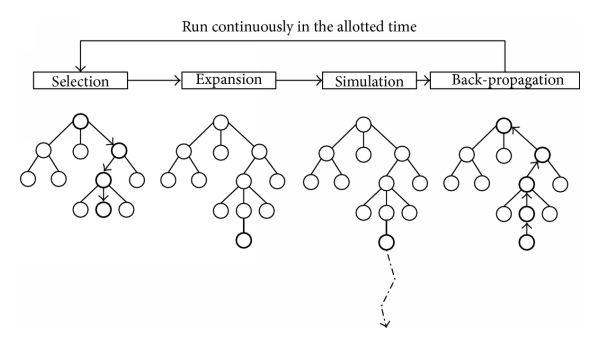
\includegraphics[width=0.5\linewidth]{report2/mcts_pic.png}
  \caption{The steps of the Monte Carlo Tree Search algorithm.\cite{MTCS_tree_pic}}
  \label{fig:preferences}
\end{figure}
\textbf{Monte Carlo Tree Search:} The root of the tree will represent the initial state of the game, in which no bid has been offered yet. Each state (node) of the game will keep information about its score (utility) and number of visits. The first bid of the agent will be a random bid with utility higher than 0.9. A \textbf{node expansion} will be performed according to a progressive widening. Meaning, if the number of visits of the parent node is greater or equal to the number of children nodes, a new relevant bid in the same space will be picked. The expansion could consist of a random bid among possible ones. However, an important observation of the early stages of the game is that both the opponent bidding model and the corresponding bidding strategy of the MCTS will be poor. Thus, we consider trying to expand using a \textbf{TIT-FOR-TAT} strategy instead of a random one. A \textbf{rollout} (simulation) will be performed using the opponent strategy model. We will consider that a leaf node is reached based on our acceptance strategy. The opponent acceptance strategy will not be used as the current approach simulates worst-case scenarios. Hence, a premature acceptance of the opponent will be beneficial. After a leaf node is reached, the \textbf{back-propagation} step will update the nodes on the upper levels with the obtained score. \textbf{Nodes selection} will be performed based on a modified version of the UCB1 formula present in Buron et al. 
\textbf{Self-Balancing Binary Tree:} If the model for the opponent bidding strategy a displays a high prediction error (see \autoref{sec:OBS}), we consider a simpler strategy. The first step of this strategy will take all the possible bids (which is less than 4000 in the party domain) and construct a \textbf{self-balancing binary tree} using the utility calculated from each bid. Therefore, each node of the tree will represent a utility score and a list of combinations that result in that utility score. Once we have this tree, we can start from the bottom-right leaves (the high utility) and bid progressively making concessions that slowly go up the tree approaching the root, but never going on the left side of the tree. Assuming a normal distribution of utility scores, the root should have a utility value close to 0.5.

\subsection{Opponent Bidding Strategy Model}
\label{sec:OBS}
A core component of MCTS is the simulation of various session rollouts. However, learning the opponents behaviour which can suddenly change is a non-trivial moving target problem.\cite{Baarslag2016} Baarslag et. al mentions several methods for learning the opponents bidding strategy.\cite{Baarslag2016} Generally divided into regression analysis and time series analysis, the latter do not assume any underlying decision function.
%The former assume that the opponent acts according to a decision function which can be captured using a set of latent probablistic variables. As there are no reasons to believe the validity of this assumption, 
% We turn to time series analysis methods, as we cannot assume that the opponents strategy can be captured by a function. 
%Some of these methods use artificial neural networks, derivatives of concession functions or markov decision processes. 
In particular, the signal processing method Gaussian Process Regression has multiple advantages. First, it does not require pretraining. Second, gaussian processes can be used for classification problems. Third, it can predict moving targets. 
%\textcolor{red}{, it can be applied to real-time negotiation settings. , it is computationally inexpensive. , it provides a measure for uncertainty in the form of variance. , it is the method proposed by several authors.} 
The aim of using GPR in this context is to estimate the opponents expected bid $y_*$ and variance $\sigma_*^2$ given an unobserved $x_*$ and an observed history of observation and opponent bid tuples ($X,Y$). Both, $y_*$ and $\sigma$, can be used to sample opponent bids in a simulation. Equations 1 and 2 describe the calculation.\cite{Buron_Guessoum_Ductor_2019}

\begin{align}
    \label{eq:GPR}
    K &= \begin{bmatrix}
    k(x_1,x_1)&\cdots &k(x_n,x_1) \\
    \vdots & \ddots & \vdots\\
    k(x_1,x_n)&\cdots &k(x_n,x_n)
    \end{bmatrix} & K_* &= [k(x_*,x_1), \cdots, k(x_*,x_n)]\\
    y_* &= K_*K^{-1}Y &\sigma_*^2 &= K_{**} - K_* K^{-1} K_*^T
\end{align}

Equation (1) describes the proximity in terms of covariance matrices $K$ and $K_*$ for features $X$ and $x_*$. Typically, $X$ reflects the time dimension alone. However, we will also consider our previous bids, opponent preferences or a combination. $K$ refers to the covariance matrix within the set of $X$, whereas $K_*$ describes the covariance vector between $x_*$ and $X$. $k(a,b)$ denotes a kernel function as proximity measure. With $Y$ being the previous bids and $y_*$ the expected bid, we can calculate $\mathbb{E}[y_*|K_*,K,Y]$ and its variance $\sigma_*^2$. By assuming that each $X$ form a multivariate Gaussian, equations in (2) follow. We choose RQF as kernel function, as it promises the best performance according to Buron et al.\cite{Buron_Guessoum_Ductor_2019} In the case of a GPR, the kernel function is used to construct the covariance matrix.
As proposed by Baarslag et. al., we will use the mean squared error (MSE) to determine the prediction error.\cite{Baarslag2016} This will guide the use of the prediction or switch to a fallback bidding strategy. As a further note, we will make the simplifying assumption that the each issue does not interact with another. Hence, we can predict the bid by predicting each issue separately. 

\subsection{Opponent Preference Model}
First, it should be noted that according to Tim Baarslag the opponent model makes a surprisingly small contribution to the performance of a negotiation strategy.\cite{Baarslag2014} However, as the HardHeaded model in ANAC 2011 showed, it had a significant impact on the outcome of the tournament and makes it reasonable to implement. Given the small yet crucial contribution, we will implement a frequency-based opponent preference model instead of a more sophisticated method such as bayesian learning. \autoref{fig:preferences} shows how frequencies within the opponent's bidding history can offer insight to its preferences. We can use these preferences as an additional input for the opponent bidding strategy model and as a way to estimate the Pareto frontier. 
Additionally, two assumptions can facilitate the preference modeling. First, the earlier bids will reflect the opponent's preference more than the later ones. Second, the opponent will concede more on issues with less importance than on issues with high importance.\cite{Baarslag2016} Thanks to the nature of the frequency-based model, these assumptions can be incorporated in the form of time-discounted frequencies or variance statistics respectively.

\begin{figure}[h!]
  \centering
  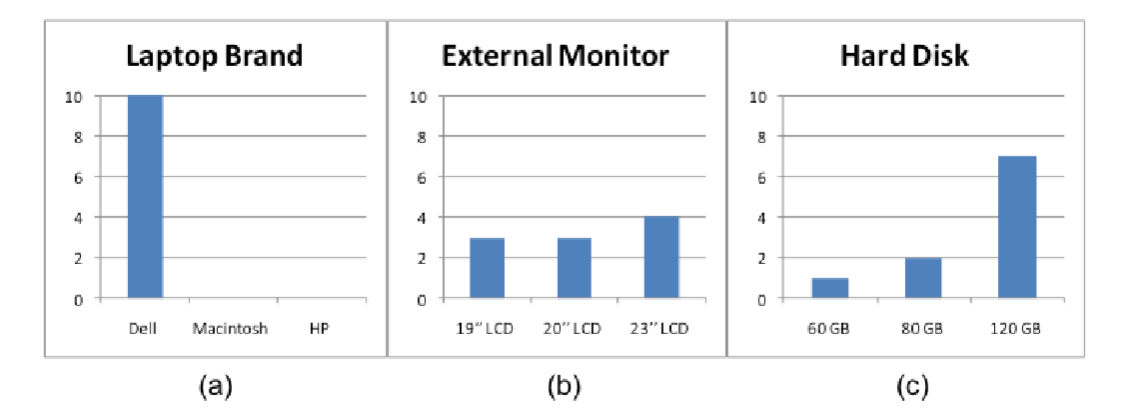
\includegraphics[width=0.75\linewidth]{report2/example_histogram.png}
  \caption{A histogram example with the last 10 offers made by the opponent agent in the Laptop domain taken from Fishel et. al.\cite{Fishel2013}}
  \label{fig:preferences}
\end{figure}


\clearpage
% \renewcommand\refname{\scriptsize References\vspace*{-4mm}}
\bibliographystyle{plain}
\bibliography{references2}

\end{document}

% 
